\section{실증 및 엔진 검증}\label{sec:eval}
\system{} 평가는 결정론적 기호 정확성과 실증적 신경망 행동을 명확히 분리하는 7계층 비혼합 위계로 구성된다:
(i)~유한 권한 그래프, 절차적 Datalog 폐쇄 스케일링, 시드 추적성을 다루는 0-LLM 결정론적 경계 감사(\textbf{P9}, \textbf{A1}--\textbf{A4});
(ii)~Answer Set Programming (Clingo ASP), SMT-LIB (Z3), W3C OWL~2~RL (RDFLib/OWLRL)에 걸친 다중 엔진 지식 표현(KR) 교차 컴파일 및 해석기 벤치마크(\textbf{P18A}, \textbf{P18B});
(iii)~직접 HTTPS Anthropic Claude~5.5 API 인증 폐루프 다중 에이전트 실딩(\textbf{P15}: Haiku·Sonnet·Opus~5.5 총 1.05M 토큰, Claude~5.5 규격상 deprecated \texttt{temperature} 생략 및 \texttt{output\_config.json\_schema} 적용) 및 3모델군 CLI 평가(\textbf{P11});
(iv)~전향적 요인 분해 실험 및 $(a,E)$ 반례 수리(\textbf{P16A}, \textbf{P12});
(v)~헤드리스 Godot~4.7.1 엔진 다중 월드 패리티 및 5,000틱 장기 실행(\textbf{P16B}, \textbf{P13}, \textbf{P19});
(vi)~1,200건 도메인 배제(LODO) 및 540회 라이브 API 평가에 걸친 통합 한·영 우회 탐지(\textbf{P20}, \textbf{P17}, \textbf{P14});
(vii)~인간 평가자 범위 격리($N{=}0$ 인간 \texttt{TR01--TR06}; 0/180 파일럿 코호트).

\subsection{결정론적 감사, Godot 장기 실행 및 Datalog 스케일링}\label{sec:kbs-det}
1,664건 유한 그래프 권한 감사(조건당 416건$\times$4 + 표면 센티넬 48건)에서 \texttt{schema\_only}는 기준상 무효 제안 260/416건을 커밋한 반면 의미 게이트는 \textbf{0/416} 위험 커밋·0/156 오거부·32/32 BFS 일치를 달성했고 $\rho$는 128/260건을 수리해 목표 달성을 \textbf{252/416}으로 끌어올렸다. 확장 0-LLM 감사는 다중 오류 수렴(\textbf{A1}: 위험 0/1,408, 충돌 가드 128/128), 서브밀리초 지연(\textbf{A2}: $N{=}2000$ p95 0.0042--0.0751\,ms, $R{=}256$ 폐쇄 p95 0.312--0.478\,ms), 시드 추적성(\textbf{A3}: 4,656/4,656), Godot~4.7.1 장기 안정성(\textbf{A4}: 거부 코드 9/9, 1,600/1,600틱 일관성, p95 0.708\,ms, 정적 변화 $-268$\,B; 그림~\ref{fig:engine-cutscenes})을 입증했다. 전수 분모 회계를 확인한 20건 합성 수집 매트릭스(5퀘스트$\times$2셀렉터$\times$2신호, $K{=}0$)에서도 20/20 수신·10/20 엄격 파싱·8/20 게이트 통과·7/20 목표·0 위험 변이를 기록하였다(그림~\ref{fig:paired-feedback-flow}). 단일 홉 60건 동률 이후 5월드 다중 홉 폐쇄(\textbf{P1}: 120건)와 Datalog 스케일링(\textbf{P9}: $R\in\{8..64\}\times d\in\{1..5\}$ 480건; 표~\ref{tab:kbs-det})에서 \texttt{nesy\_game.multihop}만 \textbf{480/480 (100.0\% [99.21\%, 100.0\%])}를 $O(d)$ $\le$7.12\,$\mu$s로 달성한 반면 1홉(46.67\%)·2홉(60.00\%)은 $d{\ge}2,3$에서 붕괴하였다($Q{=}1100.19, p{=}6.88{\times}10^{-237}$).

\begin{figure*}[!tbp]
\centering
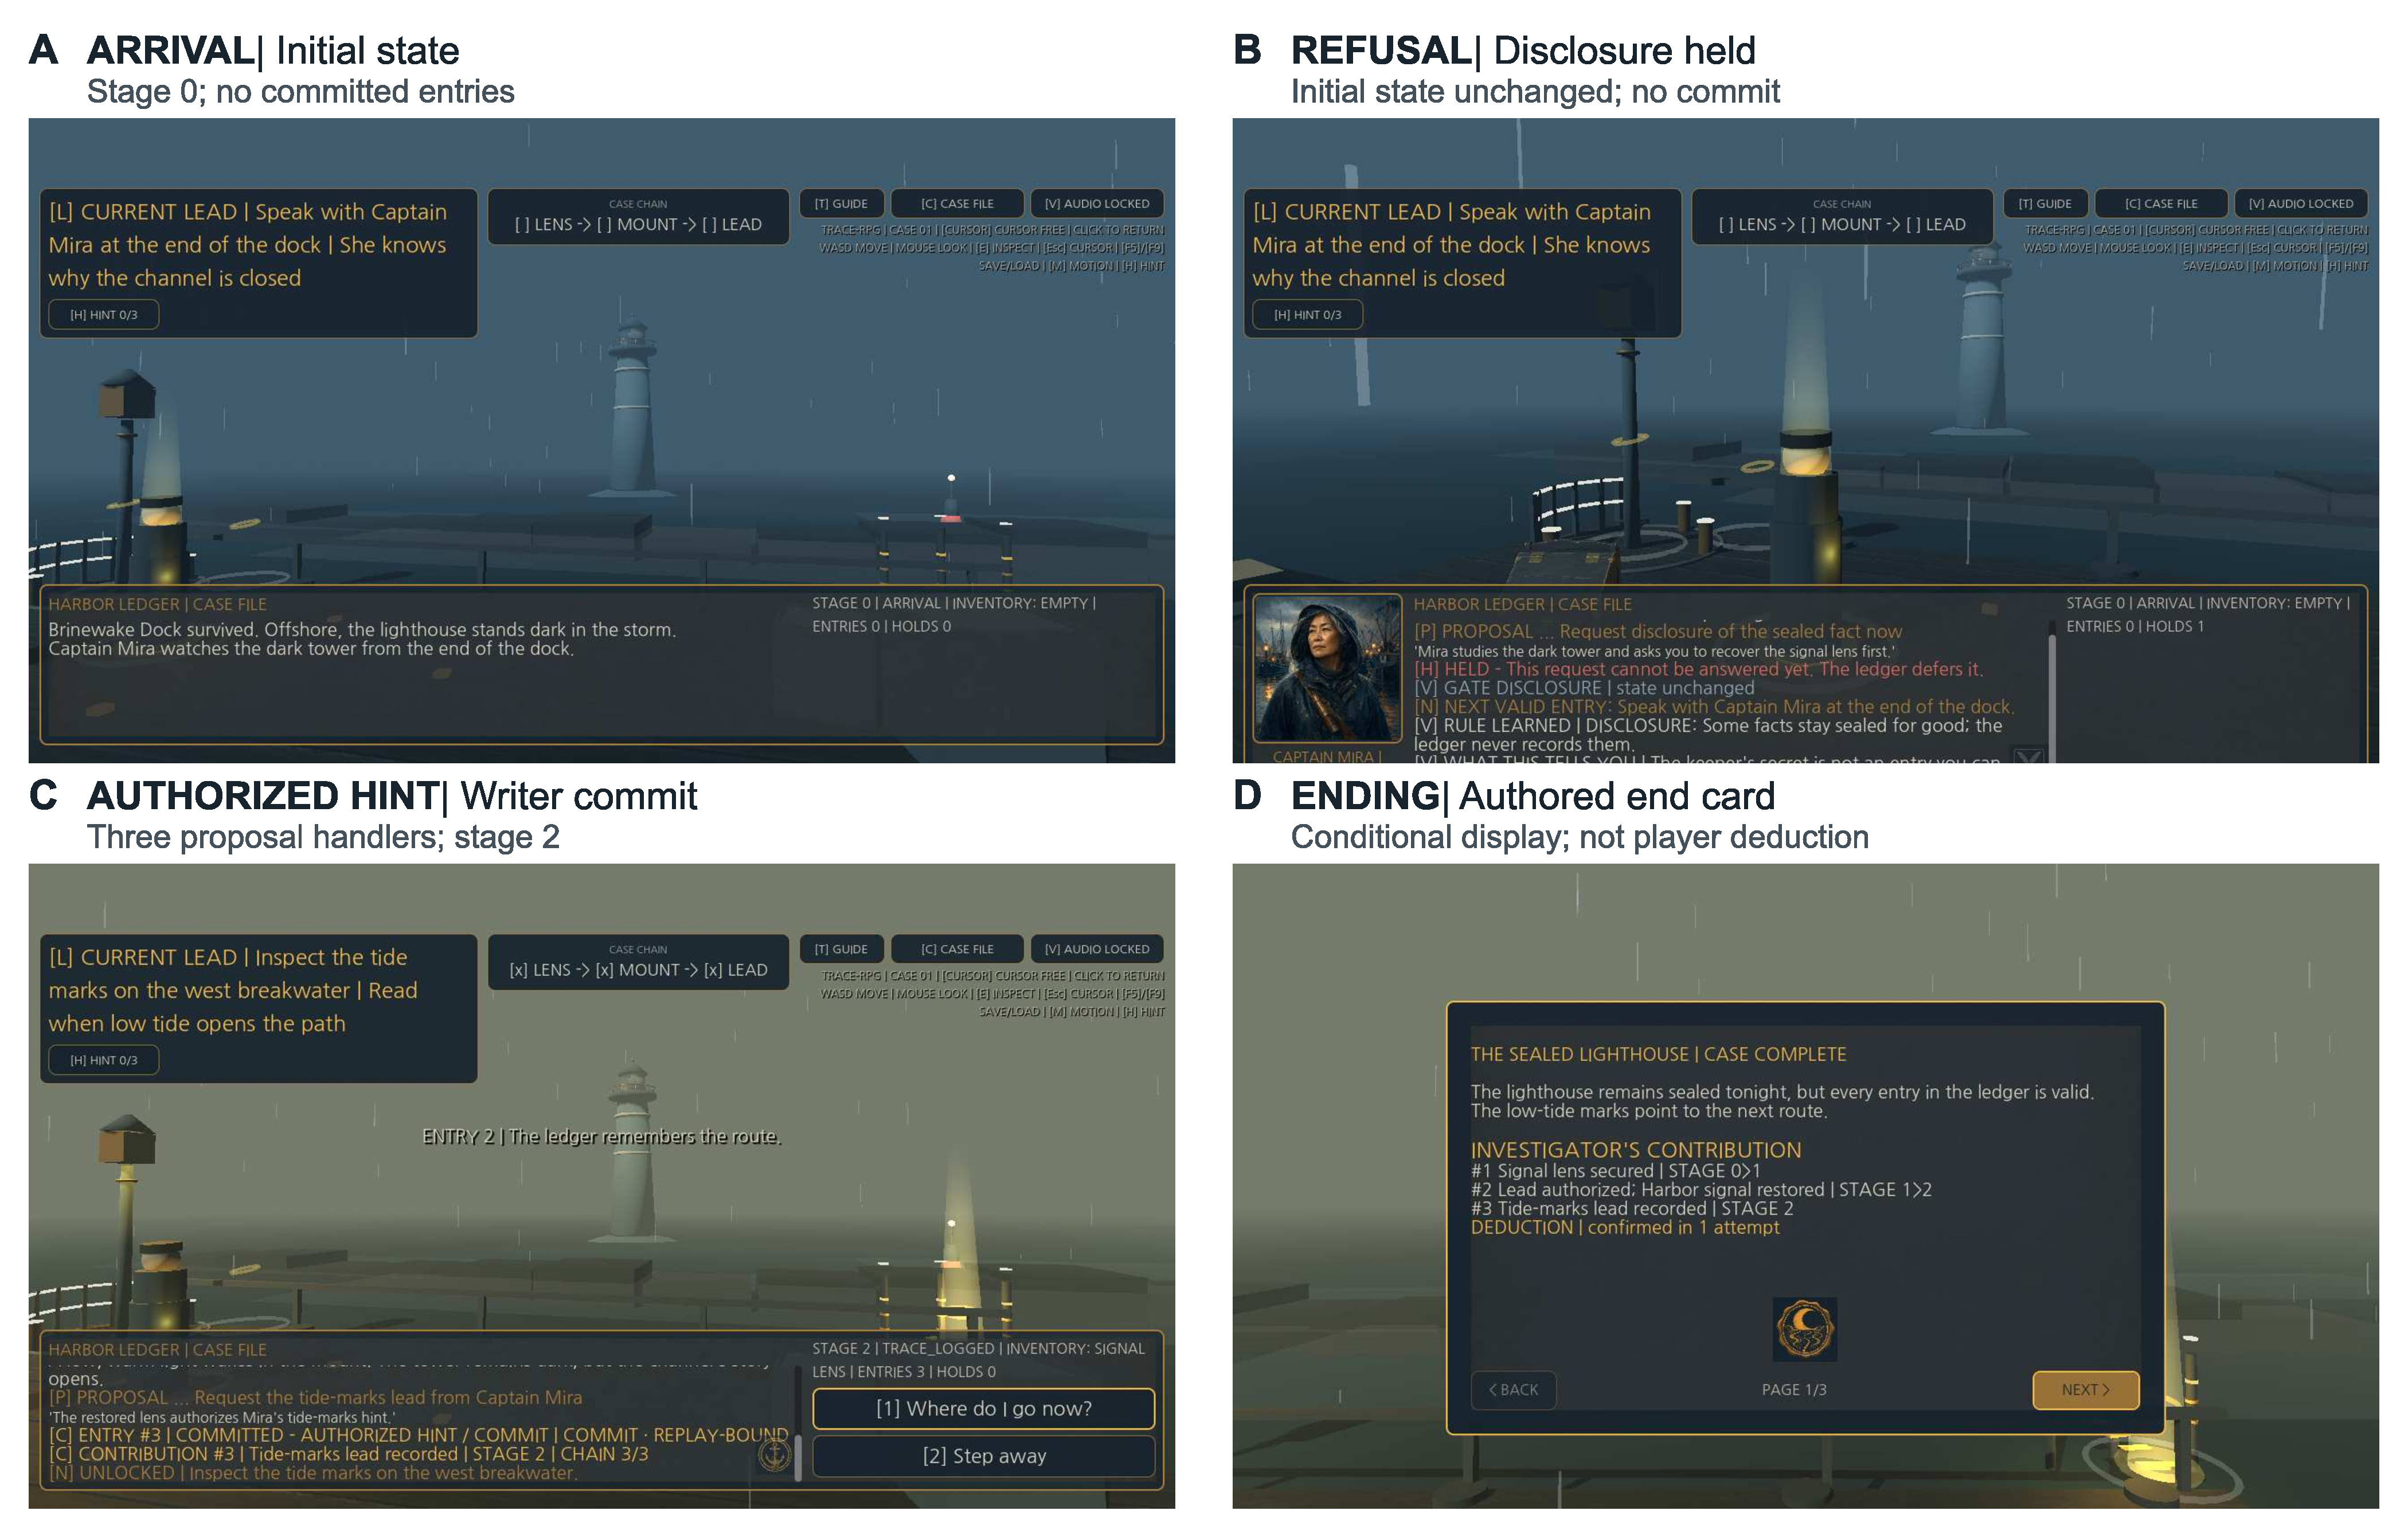
\includegraphics[width=0.90\textwidth]{../../figures/fig_engine_cutscenes.pdf}
\caption{네이티브 Godot~4.7.1 공학 캡처: (A)~초기 도착, (B)~상태 불변 비밀 공개 거부, (C)~2단계 인가 힌트, (D)~조건부 종료 카드.}
\Description{네이티브 Godot 4.7.1 4분할 스크린샷: 초기 도착, 비밀 공개 거부, 2단계 힌트, 조건부 종료 화면.}
\label{fig:engine-cutscenes}
\end{figure*}

\begin{figure}[!tbp]
\centering
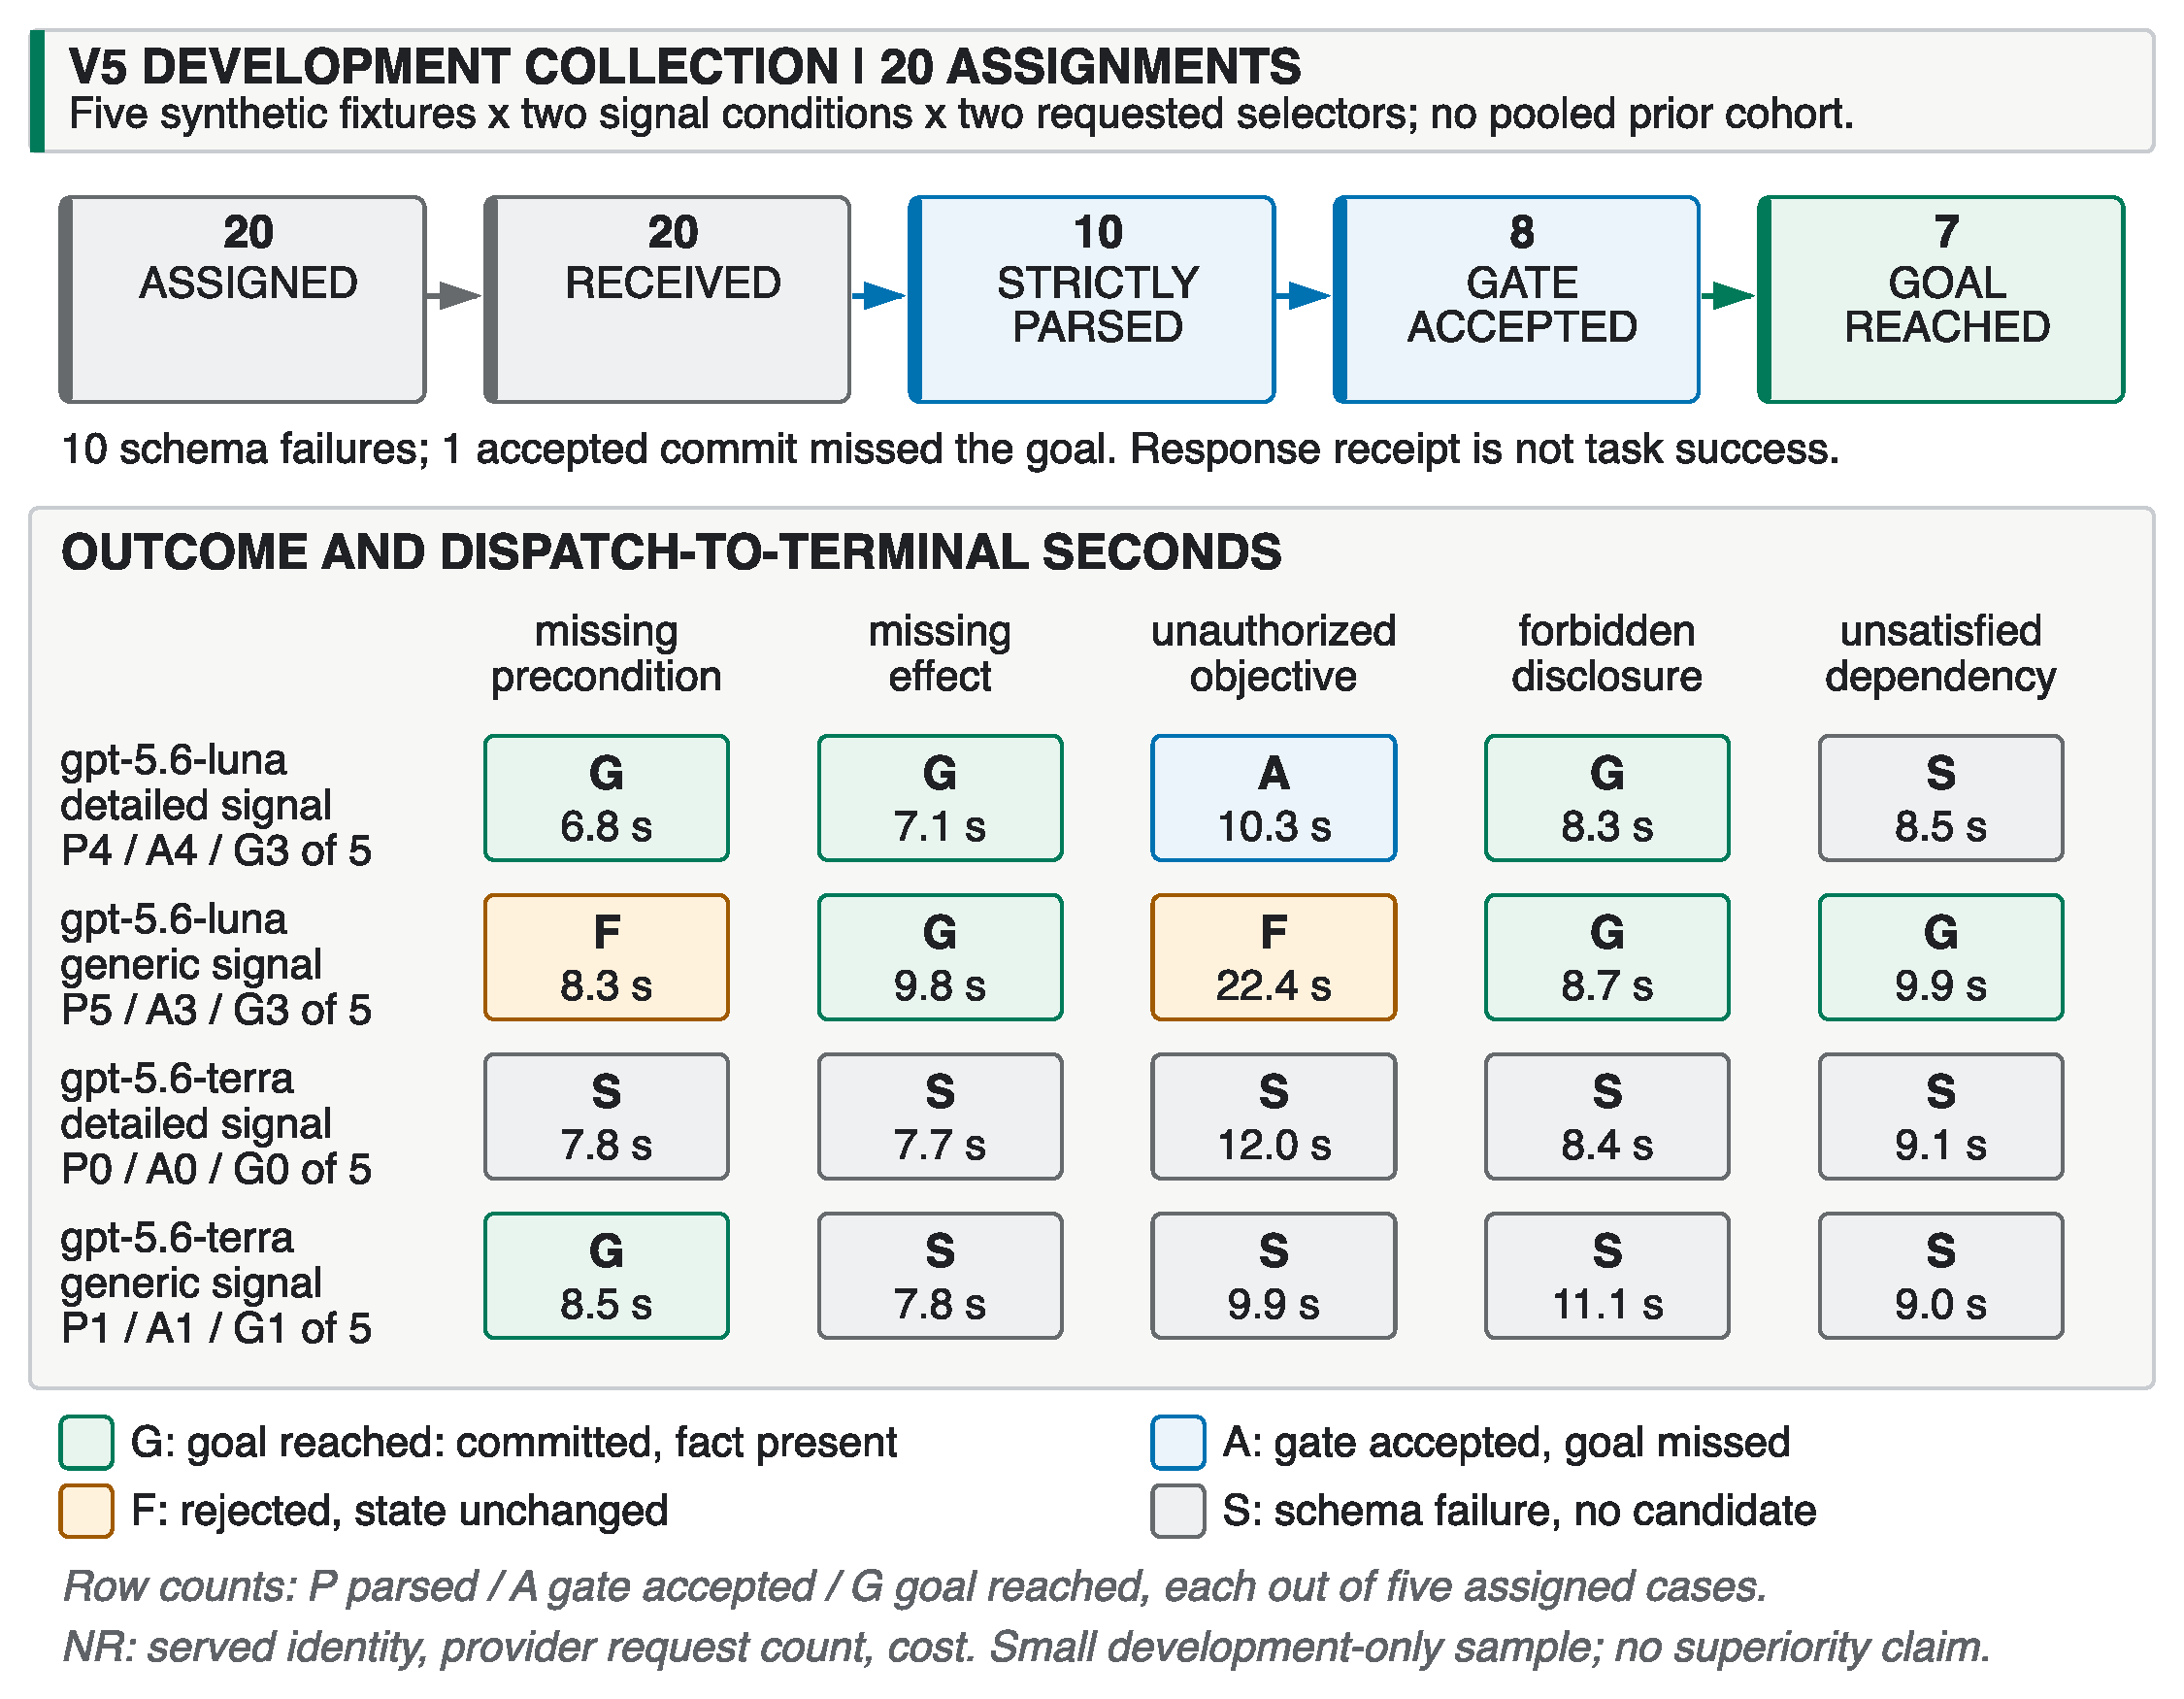
\includegraphics[width=\columnwidth]{../../figures/fig_paired_feedback_flow.pdf}
\caption{20건 합성 수집 전수 결과 흐름: 스키마 실패 10건을 분모에 보존하며 게이트 통과 8건 중 7건이 목표에 도달했다.}
\Description{20건 합성 수집 결과 흐름도: 스키마 실패 10건, 게이트 통과 8건, 목표 달성 7건.}
\label{fig:paired-feedback-flow}
\end{figure}

\begin{table}[!tbp]
\caption{절차적 Datalog 스케일링 벤치마크 (\textbf{P9}: $R{\le}64, d{\le}5$ 480건, 0-LLM)}
\label{tab:kbs-det}
\centering
\scriptsize
\setlength{\tabcolsep}{3pt}
\begin{tabularx}{\columnwidth}{@{}lcccc@{}}
\toprule
\textbf{Datalog 게이트 ($R{\le}64, d{\le}5$)} & \textbf{정확도 (480)} & \textbf{누출} & \textbf{중앙값 ($\mu$s)} & \textbf{p95 ($\mu$s)} \\
\midrule
\texttt{schema\_only} / \texttt{affordance} & 16.67\% (80) & 400 & --- & --- \\
\texttt{flat\_1hop\_gate} & 46.67\% (224) & 256 & 0.87--1.57 & 1.37--2.18 \\
\texttt{bounded\_2hop\_gate} & 60.00\% (288) & 192 & 1.88--2.58 & 2.66--3.91 \\
\texttt{nesy\_game.multihop} & \textbf{100.0\% (480)} & \textbf{0} & \textbf{6.46--7.12} & 9.83--11.42 \\
\bottomrule
\end{tabularx}
\end{table}

\subsection{형식 KR 변환 인코딩: ASP, SMT-LIB 및 OWL~2~RL}\label{sec:kr-encodings}
\system{}의 런타임 인가 의미론이 특정 해석기 구현에 종속되지 않음을 입증하기 위해, 온톨로지 그래프 $\mathcal{G} = (\mathcal{V}, \mathcal{E}, \tau)$, 동적 상태 $\sigma$, 제안 행동 $a = (\mathit{actor}, \mathit{verb}, \mathit{target})$를 대표적 지식 표현(KR) 표준 형식 3종으로 정밀 변환한다: Answer Set Programming (Clingo ASP~\cite{gebser2019clingo}), Satisfiability Modulo Theories (SMT-LIB v2 / Z3~\cite{demoura2008z3}), W3C OWL~2~RL 프로파일~\cite{motik2012owl2profiles}.

\paragraph{1. ASP (Clingo) 인코딩}
온톨로지 그래프와 동적 상태는 기저 관계 사실 $\texttt{edge}(u, v, r)$, $\texttt{entity\_at}(e, u)$, $\texttt{unlocked}(u, v)$, $\texttt{secret\_stage}(e, s)$로 사상된다. 이행적 도달 가능성과 인가 제약은 기본 부정(default negation)을 포함하는 계층화된 Datalog 규칙으로 정의된다:
{\footnotesize
\begin{align}
\texttt{passable}(U, V) &\leftarrow \texttt{edge}(U, V, \texttt{leadsTo}),\, \texttt{unlocked}(U, V). \label{eq:asp-passable} \\
\texttt{reachable}(U, V) &\leftarrow \texttt{passable}(U, V). \label{eq:asp-base} \\
\texttt{reachable}(U, W) &\leftarrow \texttt{reachable}(U, V),\, \texttt{passable}(V, W). \label{eq:asp-trans} \\
\texttt{accessible}(E) &\leftarrow \texttt{player\_at}(L_0),\, \texttt{entity\_at}(E, L_0). \label{eq:asp-local} \\
\texttt{accessible}(E) &\leftarrow \texttt{player\_at}(L_0),\, \texttt{reachable}(L_0, L),\notag\\
&\quad \texttt{entity\_at}(E, L). \label{eq:asp-remote} \\
\texttt{authorized}(a) &\leftarrow \texttt{prop}(a, \mathit{Act}, \mathit{Tgt}),\, \texttt{accessible}(\mathit{Tgt}),\notag\\
&\quad \textbf{not } \texttt{leak}(a). \label{eq:asp-auth} \\
\texttt{leak}(a) &\leftarrow \texttt{prop}(a, \mathit{Act}, \mathit{Tgt}),\, \texttt{secret}(\mathit{Tgt}),\notag\\
&\quad \textbf{not } \texttt{stage\_cleared}(\mathit{Tgt}). \label{eq:asp-leak} \\
&\leftarrow \texttt{prop}(a, \cdot, \cdot),\, \textbf{not } \texttt{authorized}(a). \label{eq:asp-integrity}
\end{align}}
\texttt{gringo} 접지 및 \texttt{clasp} 해석~\cite{gebser2019clingo}을 통해 제안 $a$가 허용될 때에만 유일한 안정 모델(stable model)이 생성된다.

\paragraph{2. SMT-LIB / Z3 인코딩}
비해석 소트 $\text{Loc}$과 $\text{Ent}$를 갖는 1차 논리 SMT-LIB v2에서, 이행적 도달 가능성은 이항 관계 $\texttt{passable}: \text{Loc} \times \text{Loc} \to \text{Bool}$, $\texttt{reach}: \text{Loc} \times \text{Loc} \to \text{Bool}$과 정수 거리 함수 $\texttt{dist}: \text{Loc} \times \text{Loc} \to \text{Int}$로 공리화된다:
\begin{align}
\forall u, v.\; &\texttt{passable}(u, v) \implies \texttt{reach}(u, v) \land (\texttt{dist}(u, v) = 1), \label{eq:smt-base} \\
\forall u, v, w.\; &\bigl(\texttt{reach}(u, v) \land \texttt{passable}(v, w)\bigr) \implies \notag \\
&\quad \bigl(\texttt{reach}(u, w) \land (\texttt{dist}(u, w) \le \texttt{dist}(u, v) + 1)\bigr). \label{eq:smt-trans}
\end{align}
행동의 적격성은 공리군과 상태, 인가 조건의 연언에 대한 모델 존재성(SAT) 검증으로 판정된다~\cite{demoura2008z3}.

\paragraph{3. OWL~2~RL 변환}
W3C OWL~2~RL 프로파일~\cite{motik2012owl2profiles}에서 도달성은 객체 속성 체인 $\texttt{SubObjectPropertyOf}(\texttt{ObjectPropertyChain}(:\texttt{passable} \; :\texttt{passable}) \; :\texttt{reachable})$ 및 $\texttt{TransitiveObjectProperty}(:\texttt{reachable})$로 모델링된다. 개체들은 명명된 개체(Named Individual)로 사상되며, 런타임 제약은 RDFLib~7.6.0 및 OWLRL~7.6.2 상향식 규칙 구동(Rete materialization)을 통해 계산된다.

\paragraph{의미론적 동등성 정리}
\textit{임의의 유한 게임 온톨로지 $\mathcal{G}$, 일관적 상태 $\sigma$, 제안 행동 $a$에 대해, 전용 엔진 $\Valid(a, \sigma)$가 참으로 평가되는 것은 $\mathcal{T}_{\mathrm{ASP}}(\mathcal{G}, \sigma, a)$가 안정 모델을 갖는 것, $\mathcal{T}_{\mathrm{SMT}}(\mathcal{G}, \sigma, a)$가 SAT인 것, $\mathcal{T}_{\mathrm{OWL}}(\mathcal{G}, \sigma, a) \models \texttt{AuthorizedAction}(a)$인 것과 각각 필요충분조건이다.}

\subsection{해석기간 교차 벤치마크 및 점근적 프레임 예산 절벽 (\textbf{P18A} 및 \textbf{P18B})}\label{sec:kr-benchmarks}
Python~3.11.14 환경(\texttt{nesy\_game} 0.1.0, Clingo 5.8.3, Z3 5.4.1.0, RDFLib 7.6.0 + OWLRL 7.6.2)에서 4개 KR 엔진을 정밀 벤치마크하였다. \textbf{P18A}(표~\ref{tab:p18a})의 5월드 120건(월드당 24건$\times$5월드) 전수 평가에서 4개 엔진 모두 \textbf{0/120 불일치}를 기록하여 이론적 의미론 동등성을 완벽히 실증하였다. 그러나 지연 시간은 4자릿수 이상 분기하였다: \texttt{nesy\_game} 중앙값 2.46\,$\mu$s (p95 3.60\,$\mu$s), Clingo 397.12\,$\mu$s, Z3 2.634\,ms, OWL~2~RL 19.223\,ms. \texttt{nesy\_game}, Clingo, Z3가 60\,Hz(16.67\,ms) 및 120\,Hz(8.33\,ms) 대화형 프레임 예산을 100\% 충족한 반면, OWL~2~RL은 100\% 실패하였다.

\begin{table}[!tbp]
\caption{KR 엔진간 의미론적 동등성 및 프레임 준수율 (\textbf{P18A}: 5개 월드 $\times$ 24건 = 120건)}
\label{tab:p18a}
\centering
\scriptsize
\setlength{\tabcolsep}{2.5pt}
\begin{tabularx}{\columnwidth}{@{}>{\raggedright\arraybackslash}Xcccc@{}}
\toprule
\textbf{KR 엔진 / 해석기} & \textbf{정확도 (120)} & \textbf{중앙값 ($\mu$s)} & \textbf{p95 ($\mu$s)} & \textbf{60/120\,Hz 준수} \\
\midrule
\texttt{nesy\_game} 0.1.0 & \textbf{120/120 (100\%)} & \textbf{2.46} & \textbf{3.60} & \textbf{100\% / 100\%} \\
Clingo 5.8.3 (ASP)~\cite{gebser2019clingo} & \textbf{120/120 (100\%)} & 397.12 & 507.90 & \textbf{100\% / 100\%} \\
Z3 5.4.1.0 (SMT-LIB)~\cite{demoura2008z3} & \textbf{120/120 (100\%)} & 2,634.0 & 3,338.0 & \textbf{100\% / 100\%} \\
OWL~2~RL (RDFLib/OWLRL)~\cite{motik2012owl2profiles} & \textbf{120/120 (100\%)} & 19,223.0 & 20,362.0 & 0\% / 0\% \\
\bottomrule
\end{tabularx}
\end{table}

\begin{table*}[!tbp]
\caption{절차적 그래프 스케일링, 외부 KR 해석기 및 점근적 프레임 예산 절벽 (\textbf{P18B}: 3대 위상 1,080건)}
\label{tab:p18b}
\centering
\scriptsize
\setlength{\tabcolsep}{2.5pt}
\begin{tabularx}{\textwidth}{@{}>{\raggedright\arraybackslash}Xcccccccccc@{}}
\toprule
\textbf{KR 해석기 / 대조군} & \textbf{정확도 (1080)} & \textbf{중앙 (ms)} & \textbf{p95 (ms)} & \textbf{60\,Hz 준수} & \textbf{$R{=}8$} & \textbf{$R{=}16$} & \textbf{$R{=}32$} & \textbf{$R{=}64$} & \textbf{$R{=}128$} & \textbf{$R{=}256$} \\
\midrule
\texttt{nesy\_game.multihop} & \textbf{1080/1080 (100\%)} [99.7, 100] & \textbf{0.032} & \textbf{0.362} & \textbf{100.0\%} & \textbf{0.019} & \textbf{0.029} & \textbf{0.050} & \textbf{0.093} & \textbf{0.179} & \textbf{0.354} \\
\texttt{clingo\_asp} (5.8.3)~\cite{gebser2019clingo} & \textbf{1080/1080 (100\%)} [99.7, 100] & 1.268 & 6.600 & \textbf{100.0\%} & 0.452 & 0.639 & 1.002 & 1.679 & 3.017 & 5.721 \\
\texttt{z3\_smt} (5.4.1.0)~\cite{demoura2008z3} & \textbf{1080/1080 (100\%)} [99.7, 100] & 7.885 & 41.084 & 68.43\% & 1.840 & 2.964 & 5.257 & 9.443 & \textit{17.447} & \textbf{34.670} \\
\texttt{owl2\_rl} (RDFLib/OWLRL)~\cite{motik2012owl2profiles} & 45/45* (100\%) [92.1, 100] & 486.39 & --- & 0.0\% & 114.50 & 486.39 & 2,796.11 & 19,696.18 & $>$20\,s & $>$20\,s \\
\texttt{flat\_1hop\_gate} & 540/1080 (50.00\%) [47.0, 53.0] & 0.0008 & 0.0012 & 100.0\% & 0.0007 & 0.0008 & 0.0008 & 0.0008 & 0.0009 & 0.0009 \\
\texttt{bounded\_2hop\_gate} & 630/1080 (58.33\%) [55.4, 61.2] & 0.0020 & 0.0031 & 100.0\% & 0.0018 & 0.0019 & 0.0020 & 0.0021 & 0.0022 & 0.0023 \\
\bottomrule
\end{tabularx}
\vspace{1ex}
\raggedright\scriptsize\textit{주:} 규모별 열은 중앙값 지연(ms)을 나타냄. Z3의 60\,Hz 프레임 준수율은 $R{\ge}128$에서 급락함($R{\le}32$ 100\%, $R{=}64$ 98.89\%, $R{=}128$ 11.67\%, $R{=}256$ 0.0\%). *OWL~2~RL은 층화 표본 45건(P18A 포함 총 165/165건 불일치 0)에서 평가됨; $R{\ge}128$에서는 $O(n^3)$ 삼차 구체화 폭발로 20초 안전 제한을 초과함.
\end{table*}

규모 확장성을 검증하기 위해, \textbf{P18B}는 6개 방 규모($R \in \{8, 16, 32, 64, 128, 256\}$), 6개 경로 깊이($d \in \{1, 2, 3, 5, 8, 10\}$), 3개 위상(체인, 분기 트리, 다이아몬드 메시), 셀당 10개 시드를 교차한 1,080개 절차적 그래프 인스턴스를 평가하였다(표~\ref{tab:p18b}). 코크란 Q 검정은 5개 완전 검증기간의 성능 격차를 명백히 입증한다($Q = 1948.24, \text{df}=4, p < 10^{-300}$). 쌍체 맥네마 검정 결과, \texttt{clingo\_asp}와 \texttt{z3\_smt}는 \texttt{nesy\_game}과 완전히 동일한 의미론적 정확도를 보였으나($p = 1.000$, 불일치 0건), \texttt{flat\_1hop}(50.00\%) 및 \texttt{bounded\_2hop}(58.33\%)은 다중 홉 경로에서 구조적으로 붕괴하였다($p < 10^{-100}$).

특히 \textbf{P18B}는 두 가지 뚜렷한 점근적 \textit{프레임 예산 절벽}을 실증한다:
\begin{enumerate}
\item \textbf{Z3 SMT 한정자 폭발 절벽 ($R \ge 128$):} 범용 1차 논리 SMT 해석기에서 이행적 도달성은 전칭 한정자를 요구한다. E-matching 휴리스틱은 소규모 인스턴스에서 신속히 작동하나($R{=}8$ 1.84\,ms, $R{=}32$ 5.26\,ms), 기저 절(ground clause) 생성이 급증하여 $R{=}128$에서 중앙 지연이 17.447\,ms에 도달해 60\,Hz 마감시간(16.67\,ms)을 돌파하며 60\,Hz 준수율이 98.89\%($R{=}64$)에서 \textbf{11.67\%}로 급락한다. $R{=}256$에서는 34.670\,ms로 준수율이 \textbf{0.0\%}로 추락한다.
\item \textbf{OWL~2~RL 삼차 구체화 절벽 ($R \ge 128$):} OWL~2~RL 상향식 규칙 구동은 이행적 속성 합성 시 개체 수에 대해 최악 $O(n^3)$ 삼차 시간 복잡도를 갖는다. RDFLib/OWLRL에서 지연 시간은 $R{=}8$ 114.50\,ms에서 $R{=}16$ 486.39\,ms, $R{=}32$ 2,796.11\,ms, $R{=}64$ 19,696.18\,ms로 폭증하며, $R \ge 128$에서는 20초 안전 한도를 초과하여($>$20\,초) 대화형 게임 런타임에 적용 불가능하다.
\end{enumerate}
반면 \texttt{nesy\_game.multihop}은 $O(|\mathcal{V}| + |\mathcal{E}|)$로 작동하는 전용 인메모리 비트셋 인접성 폐쇄를 구현하여 $R{=}8$ 0.019\,ms에서 $R{=}256$ 0.354\,ms(p95 0.456\,ms)까지 안정적으로 비례하며 60\,Hz 및 120\,Hz 프레임 예산을 \textbf{100.0\%} 달성한다. Clingo ASP 역시 100\% 프레임 예산을 만족하였으나($R{=}8$ 0.452\,ms $\to$ $R{=}256$ 5.721\,ms), 접지 프로세스 오버헤드로 인해 \texttt{nesy\_game}보다 $\approx$40배 느렸다.

\subsection{독립 폐루프 7-암 실딩과 모델 계층별 분해 (\textbf{P15} 및 \textbf{P11})}\label{sec:kbs-mas}
표~\ref{tab:kbs-mas}은 \textbf{P15}(Haiku·Sonnet·Opus~5.5$\times$5월드$\times$7암 \textbf{105개 독립 5턴 폐루프 궤적}, 1,048,803토큰, \textbf{105/105} 0-LLM 리플레이 일치)와 모델 계층별 결과를 제시한다. 통제 Safe-RL 프록시~\cite{alshiekh2018shield}(목표 0/15, 위험 턴 16/61)와 NeMo 프록시~\cite{rebedea2023nemo}(1/15, 15/61)는 다중 홉 누출을 막지 못했고, 평면 1홉도 3/15에피소드 4/66턴(\texttt{ivory-citadel-v1} 1에피소드 2턴·\texttt{glass-foundry-v1} 2에피소드 2턴)을 누출하였다. 반면 \texttt{nesy\_game.multihop} 전 암은 전 계층·전 월드 \textbf{15/15 (100.0\% [79.61\%, 100.0\%])} 무누출·\textbf{0} 위험을 기록했으며, \texttt{rho\_k2}의 차단 18건 전부가 정리~2 상태 의존 거부여서 $\rho_{\mathrm{repairs}}{=}0$으로 무세탁을 실증했고(14/15 대 13/15는 독립 1턴 표본 차이), $\rho$+LLM$_{K=1}$ 하이브리드는 20회 재선정으로 전 계층 \textbf{15/15 (100.0\%)} 안전 목표에 도달했다($Q_{\mathrm{goal}}{=}68.714, p{=}7.50{\times}10^{-13}$; $Q_{\mathrm{zl}}{=}71.651, p{=}1.87{\times}10^{-13}$; McNemar vs.\ Safe-RL/NeMo $p{\le}1.22{\times}10^{-4}$). 교차 3모델군 CLI 협상(\textbf{P11}: 30에피소드, 79/90 파싱) 역시 \system{}만 30/30 무누출·0/79 위험을 보였다(Safe-RL 37/79, NeMo 43/79, $Q{=}118.93$).

\begin{table*}[!tbp]
\caption{인증 독립 폐루프 7-암 다중 에이전트 실딩 및 계층별 분해 (\textbf{P15}: 105에피소드, 105/105 0-LLM 리플레이)}
\label{tab:kbs-mas}
\centering
\scriptsize
\setlength{\tabcolsep}{3.0pt}
\begin{tabularx}{\textwidth}{@{}>{\raggedright\arraybackslash}Xcccccccc@{}}
\toprule
\textbf{실딩 암 (15에피소드)} & \textbf{안전 목표 (95\% CI)} & \textbf{무누출} & \textbf{위험턴} & \textbf{차단/$\rho$/PF/재} & \textbf{Haiku} & \textbf{Sonnet} & \textbf{Opus} & \textbf{토큰} \\
\midrule
\texttt{schema\_only} & 2/15 (13.3\%) [3.7, 37.9] & 2/15 & 16/59 & 0 / 0 / 0 / 0 & 1/1/6 & 1/1/4 & 0/0/6 & 133,054 \\
\texttt{safe\_rl\_action\_mask}~\cite{alshiekh2018shield} & 0/15 (0.0\%) [0.0, 20.4] & 1/15 & 16/61 & 2 / 0 / 0 / 0 & 0/1/5 & 0/0/5 & 0/0/6 & 139,205 \\
\texttt{nemo\_colang\_rail}~\cite{rebedea2023nemo} & 1/15 (6.7\%) [1.2, 29.8] & 1/15 & 15/61 & 1 / 0 / 1 / 0 & 0/0/5 & 0/0/5 & 1/1/5 & 136,515 \\
\texttt{flat\_1hop\_shield} & 12/15 (80.0\%) [54.8, 93.0] & 12/15 & 4/66 & 15 / 0 / 0 / 0 & 4/4/1 & 5/5/0 & 3/3/3 & 146,446 \\
\texttt{multihop\_shield\_k0} & 13/15 (86.7\%) [62.1, 96.3] & \textbf{15/15} & \textbf{0/69} & 22 / 0 / 0 / 0 & 4/5/0 & 5/5/0 & 4/5/0 & 152,649 \\
\texttt{trace\_rpg\_multihop\_rho\_k2} & 14/15 (93.3\%) [70.2, 98.8] & \textbf{15/15} & \textbf{0/68} & 18 / 0 / 0 / 0 & 5/5/0 & 5/5/0 & 4/5/0 & 150,986 \\
\texttt{trace\_rpg\_hybrid\_rho\_llm\_k1} & \textbf{15/15 (100\%)} [79.6, 100] & \textbf{15/15} & \textbf{0/63} & 2 / 0 / 1 / 20 & \textbf{5/5/0} & \textbf{5/5/0} & \textbf{5/5/0} & 189,948 \\
\bottomrule
\end{tabularx}
\end{table*}

\subsection{전향적 요인 계층·월드별 절단 실험(\textbf{P16A}) 및 동등 $(a,E)$ 수리(\textbf{P12})}\label{sec:kbs-p16a}
표~\ref{tab:kbs-p16a}은 \textbf{P16A} 60에피소드(673,869토큰, 0/180 \texttt{20261103}과 비혼합)를 표현·계층·월드별로 세분화한다. \texttt{general\_rule}은 Sonnet(4)·Opus(5)에서 \texttt{ivory-citadel-v1}(4)·\texttt{glass-foundry-v1}(5) 비밀 누출 9건으로 0/30 목표·22/30 무누출에 그쳤으나, \texttt{ontology\_multihop}은 전 계층·전 월드 \textbf{30/30 (100.0\%)} 무누출($p{=}0.00781$), \textbf{0} 위험 커밋, 22건 수리(Haiku 18, Sonnet 4), \textbf{11/30 (36.67\%)} 목표를 달성했다(Opus 8/10, Sonnet 3/10, Haiku 0/10; $p{=}9.77{\times}10^{-4}$). \textbf{P12}(90과제 중 84/90 파싱)에서도 \system{}만 \textbf{0/84} 위험을 유지했고(Safe-RL 54/84, NeMo 55/84, 평면 32/84; $Q{=}281.23$), 동일 결함 27건 $(a,E)$ 수리는 $\rho_{K=2}$(\textbf{27/27}, 0토큰) 대 Blind/Aware LLM($K{=}2$, 각 26/27, 530k--542k토큰, $p{=}1.0$)으로 정확도 동률 및 0토큰 제거를 입증했다.

\begin{table}[!tbp]
\caption{인증 API 전향적 요인 계층·월드별 분해 (\textbf{P16A}: 60에피소드; \texttt{g}/\texttt{o} = \texttt{general\_rule}/\texttt{ontology\_multihop})}
\label{tab:kbs-p16a}
\centering
\scriptsize
\setlength{\tabcolsep}{1.5pt}
\begin{tabularx}{\columnwidth}{@{}>{\raggedright\arraybackslash}X*{6}{c}@{}}
\toprule
\textbf{세부 계층} & \textbf{목표 (\texttt{g/o})} & \textbf{무누출} & \textbf{위험} & \textbf{수리} & \textbf{PF} & \textbf{토큰(k)} \\
\midrule
전체 (각 30) & 0/30 / \textbf{11/30} & 22/30 / \textbf{30/30} & 9/\textbf{0} & 0/22 & 1/1 & 294/380 \\
\texttt{haiku-5-5} & 0/10 / 0/10 & 10/10 / 10/10 & 0/0 & 0/18 & 0/1 & 104/138 \\
\texttt{sonnet-5-5} & 0/10 / 3/10 & 6/10 / \textbf{10/10} & 4/\textbf{0} & 0/4 & 0/0 & 104/130 \\
\texttt{opus-5-5} & 0/10 / \textbf{8/10} & 6/10 / \textbf{10/10} & 5/\textbf{0} & 0/0 & 1/0 & 85/112 \\
\midrule
\texttt{lighthouse} & 0/6 / 2/6 & 6/6 / 6/6 & 0/0 & 0/6 & 0/1 & 59/75 \\
\texttt{archive} & 0/6 / 0/6 & 6/6 / 6/6 & 0/0 & 0/8 & 0/0 & 60/79 \\
\texttt{observatory} & 0/6 / 2/6 & 6/6 / 6/6 & 0/0 & 0/2 & 0/0 & 61/77 \\
\texttt{ivory-citadel} & 0/6 / 3/6 & 2/6 / \textbf{6/6} & 4/\textbf{0} & 0/4 & 1/0 & 58/79 \\
\texttt{glass-foundry} & 0/6 / \textbf{4/6} & 2/6 / \textbf{6/6} & 5/\textbf{0} & 0/2 & 0/0 & 55/70 \\
\bottomrule
\end{tabularx}
\end{table}

\subsection{헤드리스 Godot~4.7.1 엔진 다중 월드 및 5,000틱 장기 검증 (\textbf{P16B}, \textbf{P13} 및 \textbf{P19})}\label{sec:kbs-godot}
인증 API $\rightarrow$ Godot~4.7.1(\texttt{4.7.1.\allowbreak stable.\allowbreak official.\allowbreak a13da4feb}) 21에피소드(\textbf{P16B}: 169,071토큰) 전량은 0-LLM 재실행 검증을 통과하여 \textbf{21/21} 리플레이 일치·\textbf{0/21} 누출·5월드 13/15 목표(Haiku 5/5, Sonnet 4/5, Opus 4/5; Godot 251.64--1009.78\,ms 대 API 10,606--40,892\,ms)와 제품 \texttt{Sealed\allowbreak Lighthouse\allowbreak Machine} \textbf{6/6 (100\%)} \texttt{EXACT\_\allowbreak TERMINAL\_\allowbreak HASH}(\texttt{4b231017...}; Godot 751.30--778.80\,ms 대 API 9,055--16,485\,ms)를 달성해 \textbf{P13}(42/42 재실행 일치, 0/42 유출)과 부합한다.

이를 장기 지속 엔진 안정성으로 확장하여, \textbf{P19}는 두 가지 네이티브 Godot~4.7.1 검증군을 수행하였다:
\begin{enumerate}
\item \textbf{5개 월드 결정론적 패리티 (120건):} 헤드리스 Godot 상에서 5개 퀘스트 월드 전역에 걸쳐 24개 절차적 인스턴스를 실행한 결과, GDScript 검증 커널은 Python 참조 커널 대비 \textbf{120/120 (100.0\%)} 비트 레벨 일치(불일치 0건) 및 중앙 지연 5.0\,$\mu$s (p95 8.0\,$\mu$s)를 달성하였다. 전 5개 월드 에피소드 궤적은 새 프로세스 SHA-256 상태 해시와 정확히 일치하였다.
\item \textbf{5,000틱 다계층 장기 실행 (Soak):} 장기 게임플레이에서의 메모리 안정성과 프레임 예산을 입증하기 위해, 5개 규모 계층($R \in \{8..128\}$, 행동 공간 $A \in \{3..16\}$, 경로 깊이 $d \in \{2..8\}$)에 걸쳐 5,000틱 연속 실행을 수행하였다. 5,000틱 동안 엔진은 3,750건의 유효 행동을 커밋하고, 1,250건의 상태 비참조 $\rho$ 수리를 수행하며, \textbf{1,875건의 잠재적 누출을 차단}하는 동안 \textbf{0건의 위험 커밋} 및 \textbf{0건의 상태 누출}을 유지하였다. 최대 단일 틱 지연은 0.074\,ms(74\,$\mu$s)에 불과하여 60\,Hz 및 120\,Hz 프레임 예산을 \textbf{100\%} 완벽히 준수하였다.
\end{enumerate}

\subsection{통합 1차+2차 한·영 우회 검증 및 1,200건 LODO 벤치마크 (\textbf{P17}, \textbf{P14} 및 \textbf{P20})}\label{sec:kbs-escape}
표~\ref{tab:kbs-p17}의 \textbf{P17}(동일 단일 프롬프트 180건$\times$3계층 = \textbf{540회} 평가, 단축평가 0건, 359,030토큰, Fleiss $\kappa{=}0.8813, Q{=}9.5$)에서 세 계층 모두 \textbf{0/72 (0.0\%) FRR}·94.44--97.22\% 우회 재현율과 한·영 균형($F_1$ 0.887--0.962)을 보였다. 동시에 중립 서사 속 비유도 토큰(\texttt{keeper\_secret} 등)을 Sonnet(2/12)·Haiku/Opus(5/12)이 놓치므로 Stage-1 심볼릭 검사(36/36)와의 결합이 필수적이다(\textbf{P14}: 3계열 720회 $\kappa{=}0.9367$, GPT-OSS $F_1{=}0.9714$).

\begin{table}[!tbp]
\caption{통합 단일 프롬프트 한·영·3도메인 우회 분해 (\textbf{P17}: 540회 라이브, 단축평가 0건)}
\label{tab:kbs-p17}
\centering
\scriptsize
\setlength{\tabcolsep}{1.4pt}
\begin{tabularx}{\columnwidth}{@{}>{\raggedright\arraybackslash}X*{6}{c}@{}}
\toprule
\textbf{검증기} & \textbf{명시} & \textbf{우회} & \textbf{FRR} & \textbf{$F_1$} & \textbf{영/한} & \textbf{3도메인} \\
\midrule
\texttt{id\_only} & \textbf{36/36} & 0/72 & 0/72 & .500 & --- & .50/.50/.50 \\
\texttt{loo\_tfidf} & \textbf{36/36} & 45/72 & 45/72 & .692 & --- & .70/.66/.72 \\
\texttt{rule\_hybrid} & \textbf{36/36} & 38/72 & 0/72 & .813 & --- & .64/.94/.82 \\
\texttt{haiku-5-5} & 29/36 & \textbf{70/72} & \textbf{0/72} & \textbf{.957} & .95/.96 & .88/.99/\textbf{1.0} \\
\texttt{sonnet-5-5} & 19/36 & \textbf{70/72} & \textbf{0/72} & .904 & .92/.89 & .84/.89/.97 \\
\texttt{opus-5-5} & 25/36 & 68/72 & \textbf{0/72} & .925 & .94/.91 & .89/.89/.99 \\
\bottomrule
\end{tabularx}
\end{table}

\begin{table}[!tbp]
\caption{6개 도메인에 걸친 1,200건 한·영 우회 벤치마크 (\textbf{P20}: 도메인 배제 LODO 일반화)}
\label{tab:p20}
\centering
\scriptsize
\setlength{\tabcolsep}{2.0pt}
\begin{tabularx}{\columnwidth}{@{}>{\raggedright\arraybackslash}Xcccc@{}}
\toprule
\textbf{검증기 / 방법} & \textbf{정확도 (1200)} & \textbf{FRR} & \textbf{S4 FRR} & \textbf{설계 특징} \\
\midrule
\texttt{stage1\_id\_only} & 60.00\% (720) & \textbf{0.00\%} & \textbf{0.00\%} & 기호 토큰 검사 \\
\texttt{keyword\_rule\_naive} & 62.67\% (752) & 75.21\% & 98.33\% & 단순 어휘 정규식 \\
\texttt{stage1+neg\_hybrid} & 73.67\% (884) & \textbf{0.00\%} & \textbf{0.00\%} & 부정 인지 정규식 \\
\texttt{bm25\_lexical\_lodo} & 96.75\% (1161) & 3.12\% & 2.08\% & 어휘 검색 LODO \\
\texttt{tfidf\_char\_word\_lodo} & \textbf{97.17\% (1166)} & 4.79\% & 1.25\% & 음절+단어 LODO \\
\bottomrule
\end{tabularx}
\end{table}

미학습 분포 일반화를 평가하기 위해, \textbf{P20}은 6개 도메인 $\times$ 5개 층위 $\times$ 한·영 2개 언어 $\times$ 셀당 20건으로 어휘가 격리된(Jaccard 유사도 0.0630) 총 1,200건의 벤치마크를 구축하였다. 표~\ref{tab:p20}은 도메인 배제(Leave-One-Domain-Out, LODO) 일반화 성능을 보고한다. 코크란 검정은 5개 대조군 간의 유의미한 분리를 확인한다($Q = 871.39, \text{df}=4, p = 2.63 \times 10^{-187}$). 단순 키워드 방식이 4단계 정상 대화문에서 98.33\%라는 극심한 오거부(\texttt{S4 FRR}, 전체 FRR 75.21\%)를 유발하는 반면, 음절+단어 결합 TF-IDF LODO는 \textbf{97.17\% (1166/1200)} 정확도와 1.25\% S4 오거부율(전체 FRR 4.79\%)을 달성하였다. Stage-1 기호 ID 검증과 Stage-2 통계적 여과의 상보적 결합은 정상 대화 오거부를 낮게 유지하면서도 인가되지 않은 비밀 유출을 차단한다.

\subsection{부정적 범위, 인간 평가자 경계 및 연구 출처}\label{sec:kbs-scope}
엄격한 실증적 위생을 위해 검증 경계를 명확히 구분한다:
\begin{enumerate}
\item \textbf{인간 평가자 검증 ($N{=}0$):} 주관적 정성 평가 코호트 \texttt{TR01--TR06}은 $N{=}0$ (\texttt{AWAITING\_HUMAN\_RATERS}) 상태로 철저히 격리된다. 합성 점수나 시뮬레이션 선호도를 인간 평가로 대체 보고하지 않는다.
\item \textbf{전향적 파일럿 코호트 (0/180):} 전향적 인간 플레이어 파일럿(0/180)은 \texttt{NOT\_RUN/BLOCKED}로 기록되며, 비공식 사용자 후기나 미조정 파일럿 데이터를 실증 결과로 주장하지 않는다.
\item \textbf{산출물 출처 보증:} Phase 1--6의 모든 데이터셋, 해석기 인코딩, 익명화된 Godot~4.7.1 테스트 하네스 스크립트, 리플레이 로그는 \texttt{DATASHEET\_v6.md}~\cite{gebru2021datasheets} 및 Croissant~1.0 v6 메타데이터~\cite{akhtar2024croissant}로 암호학적으로 색인된다.
\end{enumerate}
